\documentclass[11pt]{article}
\usepackage{amsgen,amsmath,amstext,amsbsy,amsopn,amssymb}
%\usepackage[dvips]{graphicx,color}
\usepackage{graphicx,color}
\usepackage{graphicx,color,bm}
\usepackage{epsfig}
\usepackage{enumerate}
\usepackage{float}
\usepackage{graphicx}

%\setlength{\oddsidemargin}{0.1 in} \setlength{\evensidemargin}{-0.1
%in} \setlength{\topmargin}{-0.6 in} \setlength{\textwidth}{6.5 in}
%\setlength{\textheight}{8.5 in} \setlength{\headsep}{0.75 in}
%\setlength{\parindent}{0 in} \setlength{\parskip}{0.1 in}

\textwidth 6.3in \textheight 8.8in \topmargin -0.5truein
\oddsidemargin .15truein
\parskip .1in
\renewcommand{\baselinestretch}{1.53}  % double spaced


\newcommand{\homework}[8]{
	\pagestyle{myheadings}
	\thispagestyle{plain}
	\newpage
	\setcounter{page}{1}
	\noindent
	\begin{center}
		\framebox{
			\vbox{\vspace{2mm}
				\hbox to 6.28in { {\bf Math531:~Regression - I  \hfill} }
				\vspace{6mm}
				\hbox to 6.28in { {\Large \hfill #1 (#2)  \hfill} }
				\vspace{6mm}
				\hbox to 6.28in { {\it Instructor: #3 \hfill} }
				\hbox to 6.28in { {\it Office hours: #4  \hfill #6}}
				\vspace{2mm}}
		}
	\end{center}
	\markboth{#1}{#1}
	\vspace*{4mm}
}

% ----------------------- MATH -------------------------
\def\av{\boldsymbol a}
\def\bv{\boldsymbol b}
\def\cv{\boldsymbol c}
\def\dv{\boldsymbol d}
\def\ev{\boldsymbol e}
\def\fv{\boldsymbol f}
\def\gv{\boldsymbol g}
\def\hv{\boldsymbol h}
\def\iv{\boldsymbol i}
\def\gv{\boldsymbol j}
\def\kv{\boldsymbol k}
\def\lv{\boldsymbol l}
\def\mv{\boldsymbol m}
\def\nv{\boldsymbol n}
\def\ov{\boldsymbol o}
\def\pv{\boldsymbol p}
\def\qv{\boldsymbol q}
\def\rv{\boldsymbol r}
\def\sv{\boldsymbol s}
\def\tv{\boldsymbol t}
\def\uv{\boldsymbol u}
\def\vv{\boldsymbol v}
\def\wv{\boldsymbol w}
\def\xv{\boldsymbol x}
\def\yv{\boldsymbol y}
\def\zv{\boldsymbol z}
\def\Av{\boldsymbol A}
\def\Bv{\boldsymbol B}
\def\Cv{\boldsymbol C}
\def\Dv{\boldsymbol D}
\def\Ev{\boldsymbol E}
\def\Fv{\boldsymbol F}
\def\Gv{\boldsymbol G}
\def\Hv{\boldsymbol H}
\def\Iv{\boldsymbol I}
\def\Gv{\boldsymbol J}
\def\Kv{\boldsymbol K}
\def\Lv{\boldsymbol L}
\def\Mv{\boldsymbol M}
\def\Nv{\boldsymbol N}
\def\Ov{\boldsymbol O}
\def\Pv{\boldsymbol P}
\def\Qv{\boldsymbol Q}
\def\Rv{\boldsymbol R}
\def\Sv{\boldsymbol S}
\def\Tv{\boldsymbol T}
\def\Uv{\boldsymbol U}
\def\Vv{\boldsymbol V}
\def\Wv{\boldsymbol W}
\def\Xv{\boldsymbol X}
\def\Yv{\boldsymbol Y}
\def\Zv{\boldsymbol Z}
\def\Abf{\mathbf A}
\def\Bbf{\mathbf B}
\def\Cbf{\mathbf C}
\def\Dbf{\mathbf D}
\def\Ebf{\mathbf E}
\def\Fbf{\mathbf F}
\def\Gbf{\mathbf G}
\def\Hbf{\mathbf H}
\def\Ibf{\mathbf I}
\def\Gbf{\mathbf J}
\def\Kbf{\mathbf K}
\def\Lbf{\mathbf L}
\def\Mbf{\mathbf M}
\def\Nbf{\mathbf N}
\def\Obf{\mathbf O}
\def\Pbf{\mathbf P}
\def\Qbf{\mathbf Q}
\def\Rbf{\mathbf R}
\def\Sbf{\mathbf S}
\def\Tbf{\mathbf T}
\def\Ubf{\mathbf U}
\def\Vbf{\mathbf V}
\def\Wbf{\mathbf W}
\def\Xbf{\mathbf X}
\def\Ybf{\mathbf Y}
\def\Jbf{\mathbf J}
\def\Zbf{\mathbf Z}
\def\Am{\mathrm A}
\def\Bm{\mathrm B}
\def\Cm{\mathrm C}
\def\Dm{\mathrm D}
\def\Em{\mathrm E}
\def\Fm{\mathrm F}
\def\Gm{\mathrm G}
\def\Hm{\mathrm H}
\def\Im{\mathrm I}
\def\Gm{\mathrm J}
\def\Km{\mathrm K}
\def\Lm{\mathrm L}
\def\Mm{\mathrm M}
\def\Nm{\mathrm N}
\def\Om{\mathrm O}
\def\Pm{\mathrm P}
\def\Qm{\mathrm Q}
\def\Rm{\mathrm R}
\def\Sm{\mathrm S}
\def\Tm{\mathrm T}
\def\Um{\mathrm U}
\def\mv{\mathrm V}
\def\Wm{\mathrm W}
\def\Xm{\mathrm X}
\def\Ym{\mathrm Y}
\def\Zm{\mathrm Z}
\newcommand{\Ac}{\mathcal{A}}
\newcommand{\Bc}{\mathcal{B}}
\newcommand{\Cc}{\mathcal{C}}
\newcommand{\Dc}{\mathcal{D}}
\newcommand{\Ec}{\mathcal{E}}
\newcommand{\Fc}{\mathcal{F}}
\newcommand{\Gc}{\mathcal{G}}
\newcommand{\Hc}{\mathcal{H}}
\newcommand{\Ic}{\mathcal{I}}
\newcommand{\Jc}{\mathcal{J}}
\newcommand{\Kc}{\mathcal{K}}
\newcommand{\Lc}{\mathcal{L}}
\newcommand{\Mc}{\mathcal{M}}
\newcommand{\Nc}{\mathcal{N}}
\newcommand{\Oc}{\mathcal{O}}
\newcommand{\Pc}{\mathcal{P}}
\newcommand{\Qc}{\mathcal{Q}}
\newcommand{\Rc}{\mathcal{R}}
\newcommand{\Sc}{\mathcal{S}}
\newcommand{\Tc}{\mathcal{T}}
\newcommand{\Uc}{\mathcal{U}}
\newcommand{\Vc}{\mathcal{V}}
\newcommand{\Wc}{\mathcal{W}}
\newcommand{\Xc}{\mathcal{X}}
\newcommand{\Yc}{\mathcal{Y}}
\newcommand{\Zc}{\mathcal{Z}}
\newcommand{\alphav}{\mbox{\boldmath{$\alpha$}}}
\newcommand{\betav}{\mbox{\boldmath{$\beta$}}}
\newcommand{\gammav}{\mbox{\boldmath{$\gamma$}}}
\newcommand{\deltav}{\mbox{\boldmath{$\delta$}}}
\newcommand{\epsilonv}{\mbox{\boldmath{$\epsilon$}}}
\newcommand{\zetav}{\mbox{\boldmath$\zeta$}}
\newcommand{\etav}{\mbox{\boldmath{$\eta$}}}
\newcommand{\iotav}{\mbox{\boldmath{$\iota$}}}
\newcommand{\kappav}{\mbox{\boldmath{$\kappa$}}}
\newcommand{\lambdav}{\mbox{\boldmath{$\lambda$}}}
\newcommand{\muv}{\mbox{\boldmath{$\mu$}}}
\newcommand{\nuv}{\mbox{\boldmath{$\nu$}}}
\newcommand{\xiv}{\mbox{\boldmath{$\xi$}}}
\newcommand{\omicronv}{\mbox{\boldmath{$\omicron$}}}
\newcommand{\piv}{\mbox{\boldmath{$\pi$}}}
\newcommand{\rhov}{\mbox{\boldmath{$\rho$}}}
\newcommand{\sigmav}{\mbox{\boldmath{$\sigma$}}}
\newcommand{\tauv}{\mbox{\boldmath{$\tau$}}}
\newcommand{\upsilonv}{\mbox{\boldmath{$\upsilon$}}}
\newcommand{\phiv}{\mbox{\boldmath{$\phi$}}}
\newcommand{\varphiv}{\mbox{\boldmath{$\varphi$}}}
\newcommand{\chiv}{\mbox{\boldmath{$\chi$}}}
\newcommand{\psiv}{\mbox{\boldmath{$\psi$}}}
\newcommand{\omegav}{\mbox{\boldmath{$\omega$}}}
\newcommand{\Sigmav}{\mbox{\boldmath{$\Sigma$}}}
\newcommand{\Lambdav}{\mbox{\boldmath{$\Lambda$}}}
\newcommand{\Deltav}{\mbox{\boldmath{$\Delta$}}}
\newcommand{\Omegav}{\mbox{\boldmath{$\Omega$}}}
\newcommand{\varepsilonv}{\mbox{\boldmath{$\varepsilon$}}}

\newcommand{\eps}{\varepsilon}
\newcommand{\epsv}{\mbox{\boldmath{$\varepsilon$}}}

\def\1v{\mathbf 1}
\def\0v{\mathbf 0}
\def\Id{\mathbf I} % identity matrix
\newcommand{\ind}[1]{\mathbbm{1}_{\left[ {#1} \right] }}
\newcommand{\Ind}[1]{\mathbbm{1}_{\left\{ {#1} \right\} }}
\newcommand\indep{\protect\mathpalette{\protect\independenT}{\perp}}\def\independenT#1#2{\mathrel{\rlap{$#1#2$}\mkern2mu{#1#2}}}
\newcommand{\QED}{\begin{flushright} {\bf QED} \end{flushright}}
\newcommand{\R}{\mathbb R}
\newcommand{\Real}{\mathbb R}
\newcommand{\C}{\mathbb C}
\newcommand{\E}{\mathbb E}
\newcommand{\sgn}{\mathop{\mathrm{sign}}}
\def\Pr{\mathrm P}
\def\pr{\mathrm P}
\newcommand{\Var}{\mathop{\rm Var}}
\newcommand{\var}{\mathop{\rm Var}}
\newcommand{\Cov}{\mathop{\rm Cov}}
\newcommand{\cov}{\mathop{\rm Cov}}
\newcommand{\Corr}{\mathop{\rm Corr}}
\newcommand{\ang}{\mathop{\rm Angle}}
\newcommand{\tr}{\mathop{\rm trace}}
\newcommand{\proj}{\mathop{\rm Proj}}
\newcommand{\rank}{\mathop{\rm rank}}

\newcommand{\diag}{\mathop{\rm diag}}
\newcommand{\Diag}{\mathop{\rm diag}}
\newcommand{\sk}{\vspace{0.5cm}}
\newcommand{\ds}{\displaystyle}
\newcommand{\mb}{\mbox}
\newcommand{\wh}{\widehat}
\newcommand{\argmin}{\operatornamewithlimits{argmin}}
\newcommand{\argmax}{\operatornamewithlimits{argmax}}

\newcommand{\norm}[1]{\|#1\|}
\newcommand{\abs}[1]{\left\vert#1\right\vert}
\newcommand{\set}[1]{\left\{#1\right\}}

\newcommand{\To}{\longrightarrow}

\def\equalLaw{\stackrel{\mathcal{L}}{=}}
\def\equallaw{\stackrel{\mathcal{L}}{=}}

\def\half{\frac{1}{2}}

\usepackage{caption}

\begin{document}

\begin{title}
	{\Large\bf Homework 6, MATH 455: Due Mon, 04/16/2018}
\end{title}

\author{\bf Your Name: Alexander Van Roijen}

\maketitle
{\bf Instructions}:  The homework assignment editing this \LaTeX\ document.  Download the \LaTeX\ source from the class web page and study
it to learn more about \LaTeX.  Replace the text with appropriate information.  Run ``pdflatex'' on this document.

You will submit this assignment in two parts:
\begin{enumerate}
\item Print out the PDF file and bring it to class, and
\item Send an e-mail to:
\begin{center}
gang@math.binghamton.edu
\end{center}
\emph{before class} on the due date with two attachments:
\begin{itemize}
\item The \LaTeX\ source file, and
\item The generated PDF document.
\end{itemize}
\end{enumerate}
\newpage
Please complete the following:\\
NOTE: Information has been deprecated to save paper and space, more details can be found in the R code.
\begin{enumerate}
\item  Finish R exercises 5.1, 9.1(a-d), 9.2, 9.3,9.5 of the textbook. Submit your
answers for {\color{red}ALL} questions.\\
\item 5.1
\begin{verbatim}
	> print(summary(initModel))
	
	Call:
	lm(formula = gamble ~ sex, data = teengamb)
	
	Residuals:
	Min      1Q  Median      3Q     Max 
	-29.775 -18.325  -3.766   6.334 126.225 
	
	Coefficients:
	Estimate Std. Error t value Pr(>|t|)    
	(Intercept)   29.775      5.498   5.415 2.28e-06 ***
	sex          -25.909      8.648  -2.996  0.00444 ** 
	---
	Signif. codes:  0 ‘***’ 0.001 ‘**’ 0.01 ‘*’ 0.05 ‘.’ 0.1 ‘ ’ 1
	
	Residual standard error: 29.09 on 45 degrees of freedom
	Multiple R-squared:  0.1663,	Adjusted R-squared:  0.1478 
	F-statistic: 8.977 on 1 and 45 DF,  p-value: 0.004437
	
	print(coef(exhaustive,1:dim(X)[1]))
	[[1]]
	(Intercept)         sex      income 
	4.040829  -21.634391    5.171584 
	[[2]]
	(Intercept)         sex      status 
	60.2232938 -35.7093699  -0.5855441 
	[[3]]
	(Intercept)         sex      verbal 
	60.661923  -27.722083   -4.527926 
	[[4]]
	(Intercept)         sex      income      verbal 
	24.138972  -22.960220    4.898090   -2.746817 
	[[5]]
	(Intercept)         sex      status      income 
	13.0314758 -24.3393433  -0.1495854   4.9279770 
	[[6]]
	(Intercept)         sex      status      verbal 
	69.2216451 -33.7520159  -0.4039186  -2.7036680 
	[[7]]
	(Intercept)          sex       status       income       verbal 
	22.55565063 -22.11833009   0.05223384   4.96197922  -2.95949350 
	
	...a few samples

	Call:
	lm(formula = gamble ~ sex, data = teengamb)
	
	Coefficients:
	Estimate Std. Error t value Pr(>|t|)    
	(Intercept)   29.775      5.498   5.415 2.28e-06 ***
	sex          -25.909      8.648  -2.996  0.00444 ** 

	Call:
	lm(formula = gamble ~ sex + income, data = teengamb)

	Coefficients:
	Estimate Std. Error t value Pr(>|t|)    
	(Intercept)    4.041      6.394   0.632  0.53070    
	sex          -21.634      6.809  -3.177  0.00272 ** 
	income         5.172      0.951   5.438 2.24e-06 ***

	Call:
	lm(formula = gamble ~ sex + income + verbal, data = teengamb)
	
	Coefficients:
	Estimate Std. Error t value Pr(>|t|)    
	(Intercept)  24.1390    14.7686   1.634   0.1095    
	sex         -22.9602     6.7706  -3.391   0.0015 ** 
	income        4.8981     0.9551   5.128 6.64e-06 ***
	verbal       -2.7468     1.8253  -1.505   0.1397  	
\end{verbatim}

\begin{figure}[H]
	\centering
	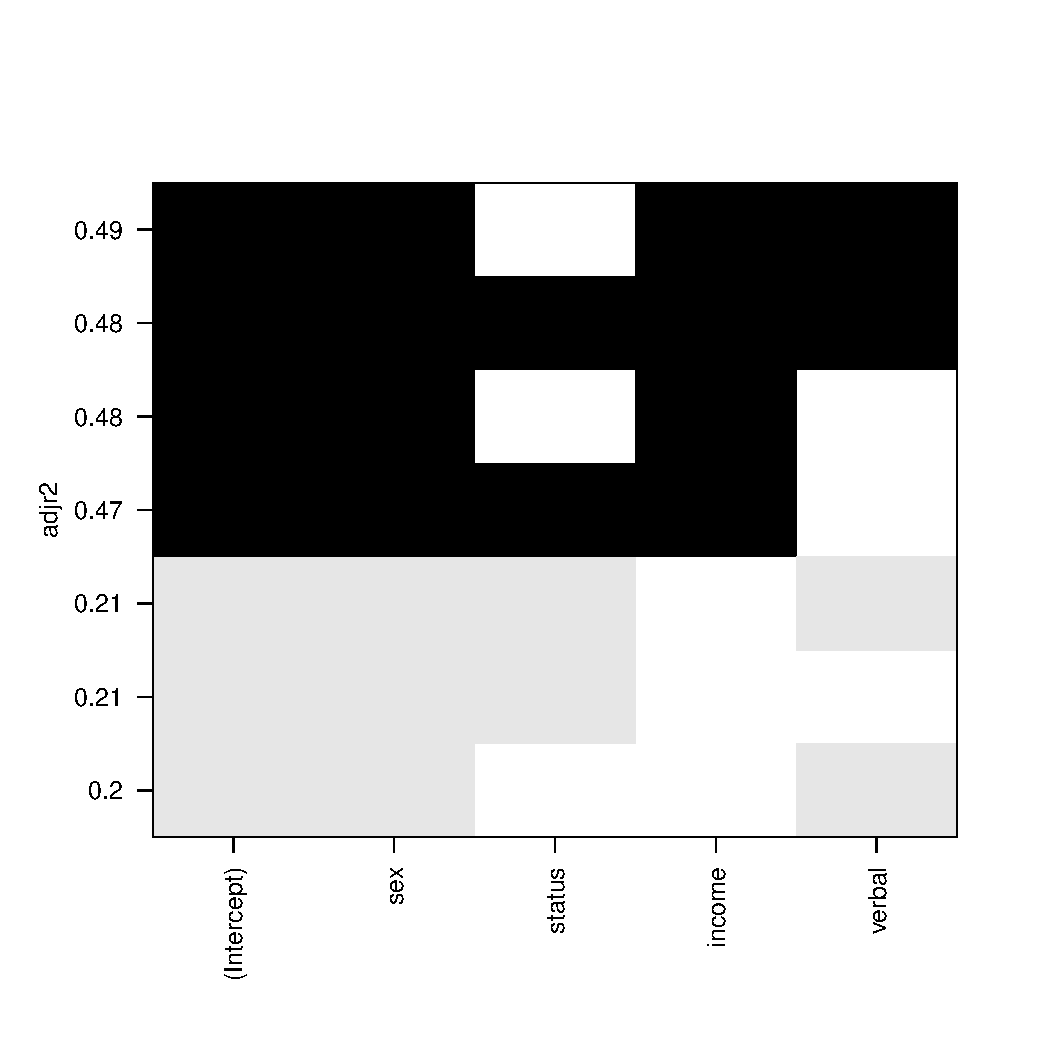
\includegraphics[width=15cm,height=15cm]{teenGambDiv}
	\caption[teengambDiv]{adjR2 values from various models}
	\label{teenGamb}
\end{figure}

As we can see, there are some general trends. Sex always seems to have a negative coefficient and be significant. Further, verbal also tends to be negative. Meanwhile status fluctuates around positive and negative. However, as to be expected, when there are less predictors in the model, there will be more significance to sex. This can be seen in a higher std error with the sex predictor given more predictors. Thus, some of its explanatory power is lost as we add more parameters.

\item 9.1
\begin{enumerate}
	\item 
	\begin{figure}[H]
		\centering
		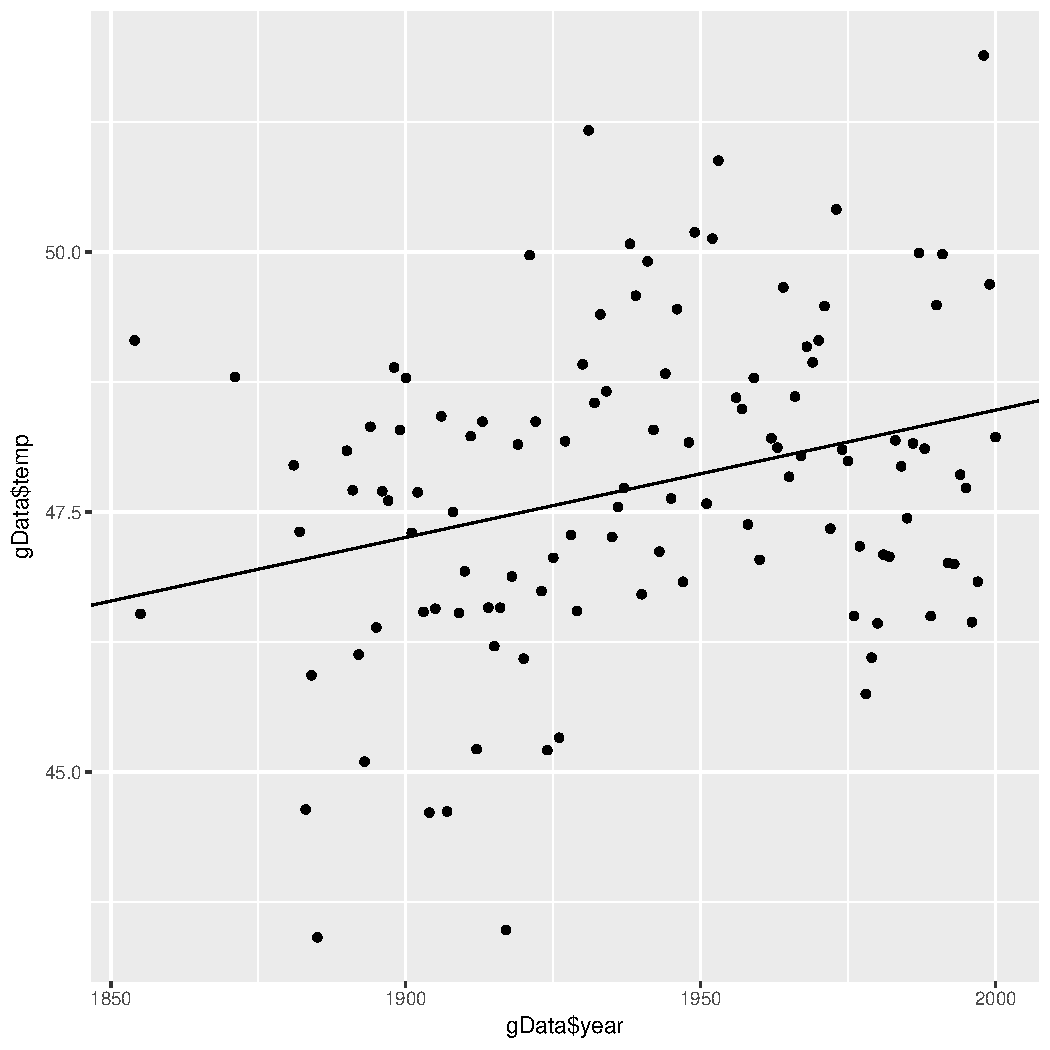
\includegraphics[width=10cm,height=10cm]{mayblin}
		\caption[mayblin]{we see a general yet scattered linear trend }
		\label{aadata}
	\end{figure}
	clearly, there is a minute increase over the years on average. This is not a certainty but appears to be present.
	\item
	\begin{verbatim}
		tempsOG = gData$temp[2:length(gData$temp)]
		tempsPrev = gData$temp[1:length(gData$temp)-1]
		cor(x=tempsOG,y=tempsPrev)
		>0.2554538
	\end{verbatim}
	Looking at this information, we see there is some, but not much, correlation between each year, however, the linear trend is not very strong to begin with, so it puts some question on the strength of the relation.
	\item
	now lets look at a ten degree polynomial utilizing the poly function
	\begin{verbatim}
		c> tendeg = lm(temp~poly(year,10),gData)
		> summary(tendeg)
		
		Call:
		lm(formula = temp ~ poly(year, 10), data = gData)
		
		Coefficients:
		Estimate Std. Error t value Pr(>|t|)    
		(Intercept)       47.7426     0.1319 361.927  < 2e-16 ***
		poly(year, 10)1    4.7616     1.4146   3.366  0.00107 ** 
		poly(year, 10)2   -0.9071     1.4146  -0.641  0.52277    
		poly(year, 10)3   -3.3132     1.4146  -2.342  0.02108 *  
		poly(year, 10)4    2.4383     1.4146   1.724  0.08774 .  
		poly(year, 10)5    3.3824     1.4146   2.391  0.01860 *  
		poly(year, 10)6    1.2124     1.4146   0.857  0.39337    
		poly(year, 10)7   -0.9373     1.4146  -0.663  0.50908    
		poly(year, 10)8   -1.1011     1.4146  -0.778  0.43812    
		poly(year, 10)9    1.3994     1.4146   0.989  0.32483    
		poly(year, 10)10   0.3474     1.4146   0.246  0.80652    
	\end{verbatim}
	So we look at the five degree polynomial in more detail 
	\begin{verbatim}
		> fivedeg=lm(temp~year+I(year^2)+I(year^3)+I(year^4)+I(year^5),gData)
		> summary(fivedeg)
		
		Call:
		lm(formula = temp ~ year + I(year^2) + I(year^3) + I(year^4) + 
		I(year^5), data = gData)

		Coefficients: (1 not defined because of singularities)
		Estimate Std. Error t value Pr(>|t|)  
		(Intercept)  1.497e+06  8.553e+05   1.750   0.0829 .
		year        -3.086e+03  1.775e+03  -1.739   0.0849 .
		I(year^2)    2.385e+00  1.381e+00   1.727   0.0869 .
		I(year^3)   -8.189e-04  4.773e-04  -1.716   0.0890 .
		I(year^4)    1.054e-07  6.186e-08   1.704   0.0912 .
		I(year^5)           NA         NA      NA       NA  
	\end{verbatim}
	So, now we see that the 4 degree polynomial is just as good, so we reduce it.
	\begin{verbatim}
	> fourdeg=lm(temp~year+I(year^2)+I(year^3)+I(year^4),gData)
	> summary(fourdeg)
	
	Call:
	lm(formula = temp ~ year + I(year^2) + I(year^3) + I(year^4), 
	data = gData)
	
	Residuals:
	Min      1Q  Median      3Q     Max 
	-4.0085 -0.9618 -0.0913  0.9926  3.7370 
	
	Coefficients:
	Estimate Std. Error t value Pr(>|t|)  
	(Intercept)  1.497e+06  8.553e+05   1.750   0.0829 .
	year        -3.086e+03  1.775e+03  -1.739   0.0849 .
	I(year^2)    2.385e+00  1.381e+00   1.727   0.0869 .
	I(year^3)   -8.189e-04  4.773e-04  -1.716   0.0890 .
	I(year^4)    1.054e-07  6.186e-08   1.704   0.0912 .
	---
	Signif. codes:  0 ‘***’ 0.001 ‘**’ 0.01 ‘*’ 0.05 ‘.’ 0.1 ‘ ’ 1
	
	Residual standard error: 1.431 on 110 degrees of freedom
	Multiple R-squared:  0.1522,	Adjusted R-squared:  0.1213 
	F-statistic: 4.936 on 4 and 110 DF,  p-value: 0.001068
	
	\end{verbatim}
	However, our results arent significant, we reduce it once more and plot the results
	\begin{figure}[H]
		\centering
		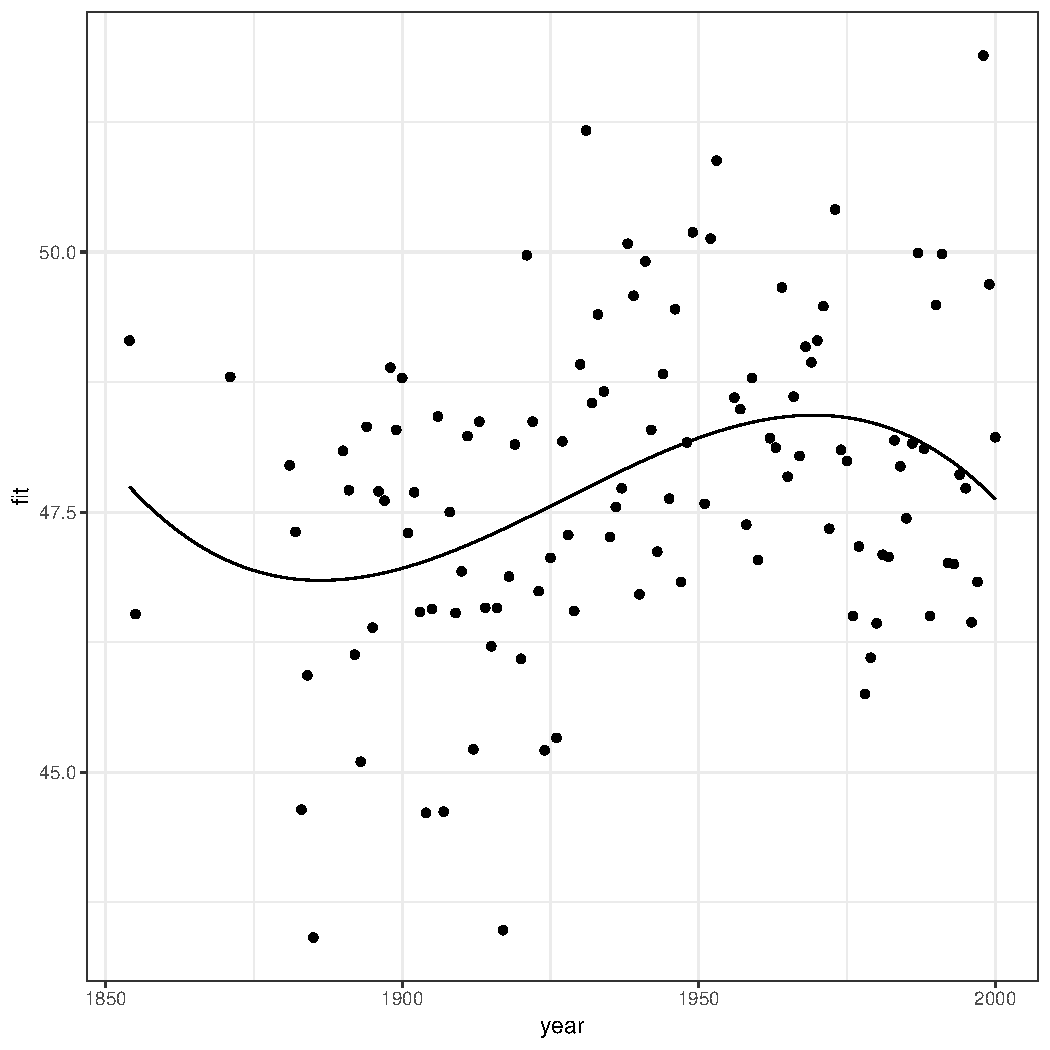
\includegraphics[width=10cm,height=10cm]{newTrend}
		\caption[newTrend]{a three degree polynomial following the data decently well}
		\label{aadatapt2}
	\end{figure}
	We now predict the temperature in 2020
	\begin{verbatim}
		> predict(threedeg,new=data.frame(year=2020),interval="prediction")
		fit      lwr      upr
		1 45.9456 42.17797 49.71322
	\end{verbatim}
	\item
	Now, looking at a segmented analysis, we get the following
	\begin{figure}[H]
		\centering
		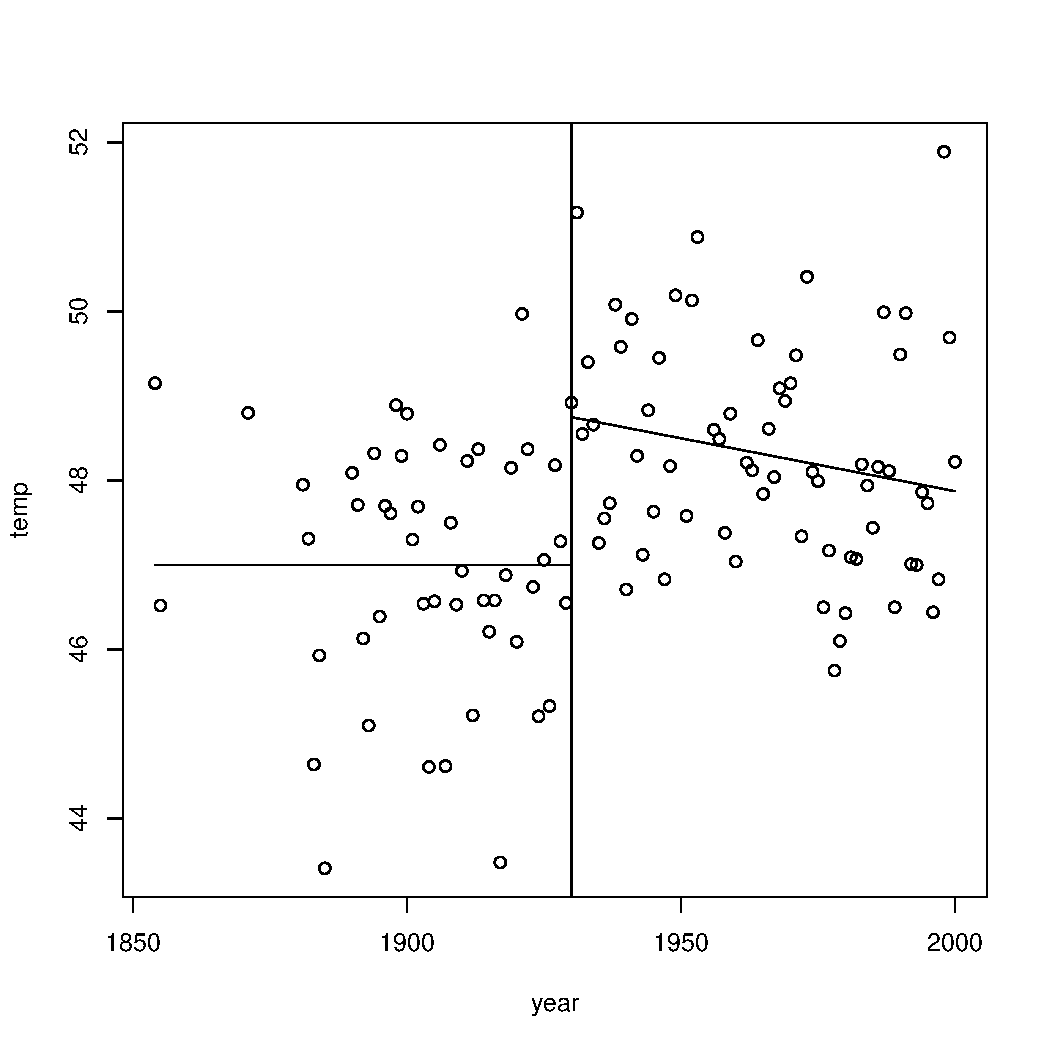
\includegraphics[width=10cm,height=10cm]{segmented}
		\caption[newTrend]{a segmented diagram of our regression}
		\label{aadatapt3}
	\end{figure}
	
	Looking at this image, to claim the temperature was constant until 1930 does not make much sense. As we can see, there would be a very sudden jump in temperatures suddenly going into the 1930s. It would make more sense for there to have been a gradual increase going into the 1930s or something of the like.
	
	More details can be found in the R code of how this was constructed.
\end{enumerate}
\item 9.2
First, we check if there is any signifigant way to improve our resposne variable.
	\begin{figure}[H]
		\centering
		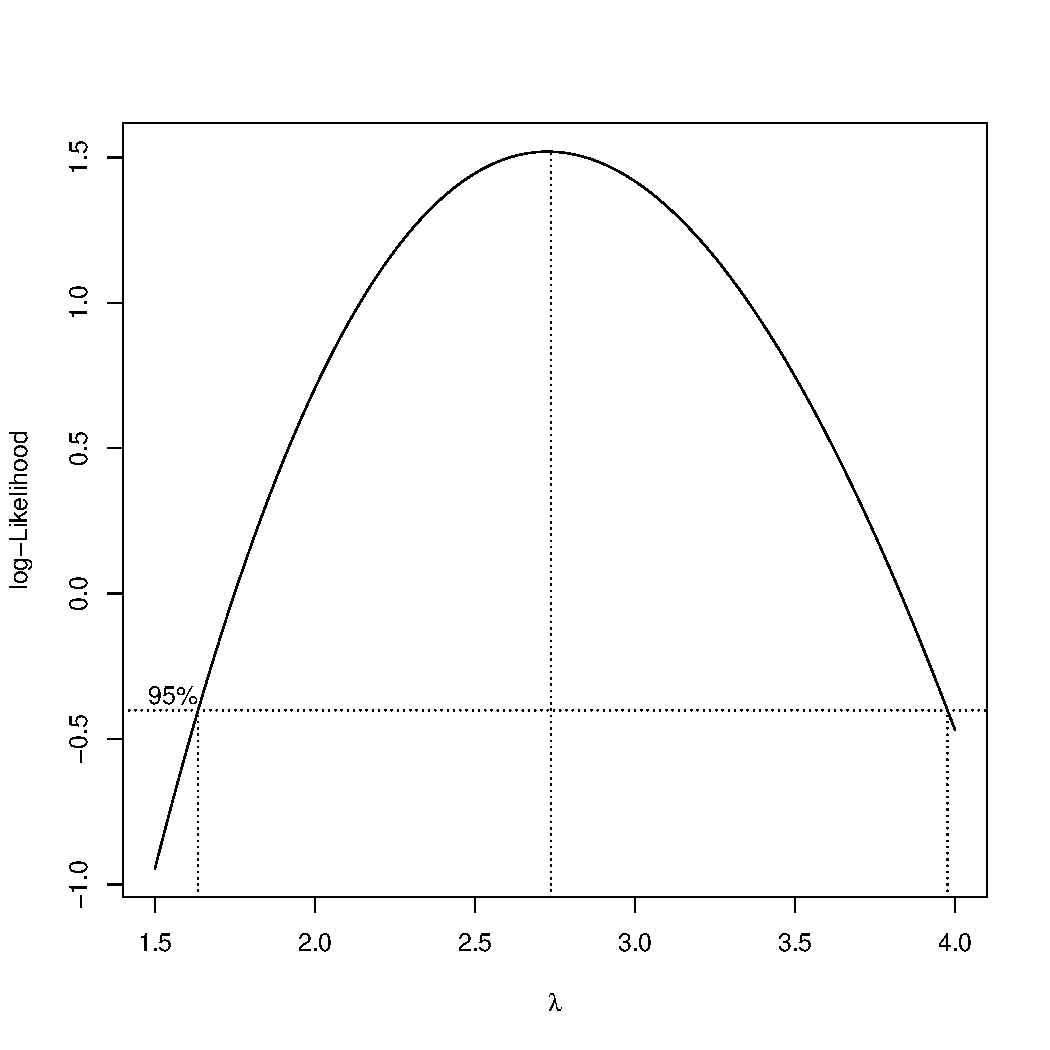
\includegraphics[width=10cm,height=10cm]{bxcx}
		\caption[corn]{box cox potential for our response}
		\label{corndata}
	\end{figure}
We see there is quite a good argument here to modify our response variable. In this situation, for interpretability, we let lambda equal 3 and apply it.
\begin{verbatim}

> nCornm = lm(((I(yield^3)-1)/3)~nitrogen,cData)
> summary(nCornm)

Call:
lm(formula = ((I(yield^3) - 1)/3) ~ nitrogen, data = cData)

Residuals:
Min      1Q  Median      3Q     Max 
-455013 -190004    1157  175247  605739 

Coefficients:
Estimate Std. Error t value Pr(>|t|)    
(Intercept) 489620.0    62248.8   7.866 8.63e-10 ***
nitrogen      2425.9      450.5   5.385 3.03e-06 ***
---
Signif. codes:  0 ‘***’ 0.001 ‘**’ 0.01 ‘*’ 0.05 ‘.’ 0.1 ‘ ’ 1

Residual standard error: 273900 on 42 degrees of freedom
Multiple R-squared:  0.4084,	Adjusted R-squared:  0.3943 
F-statistic: 28.99 on 1 and 42 DF,  p-value: 3.029e-06

> summary(cornMod)

Call:
lm(formula = yield ~ nitrogen, data = cData)

Residuals:
Min      1Q  Median      3Q     Max 
-60.439 -10.939   1.534  14.082  29.697 

Coefficients:
Estimate Std. Error t value Pr(>|t|)    
(Intercept) 107.43864    4.66622   23.02  < 2e-16 ***
nitrogen      0.17730    0.03377    5.25 4.71e-06 ***
---
Signif. codes:  0 ‘***’ 0.001 ‘**’ 0.01 ‘*’ 0.05 ‘.’ 0.1 ‘ ’ 1

Residual standard error: 20.53 on 42 degrees of freedom
Multiple R-squared:  0.3962,	Adjusted R-squared:  0.3818 
F-statistic: 27.56 on 1 and 42 DF,  p-value: 4.713e-06
	
\end{verbatim}
looking at these two models, we see an improved R squared and adjusted R squared values, which indicated a rough but overall better goodness of fit.
\\
I also checked to see if a broken stick regression would work well, but there is no apparent split within the data. However, it does seem non linear, so a quadratic model may work well.
\begin{verbatim}
	> nCornm2 = lm(yield~nitrogen+I(nitrogen^2),cData)
	> summary(nCornm2)
	
	Call:
	lm(formula = yield ~ nitrogen + I(nitrogen^2), data = cData)
	
	Residuals:
	Min      1Q  Median      3Q     Max 
	-47.162  -7.092   0.368  10.058  26.571 
	
	Coefficients:
	Estimate Std. Error t value Pr(>|t|)    
	(Intercept)   94.1620969  4.4067757  21.368  < 2e-16 ***
	nitrogen       0.5794901  0.0800285   7.241 7.54e-09 ***
	I(nitrogen^2) -0.0014831  0.0002787  -5.321 3.97e-06 ***
	---
	Signif. codes:  0 ‘***’ 0.001 ‘**’ 0.01 ‘*’ 0.05 ‘.’ 0.1 ‘ ’ 1
	
	Residual standard error: 15.98 on 41 degrees of freedom
	Multiple R-squared:  0.6428,	Adjusted R-squared:  0.6254 
	F-statistic:  36.9 on 2 and 41 DF,  p-value: 6.817e-10
\end{verbatim}
We see even more improvement in our data, going further, a cubed term does not seem to aid much, so we stop here.
\item 9.3

\begin{figure}[H]
	\centering
	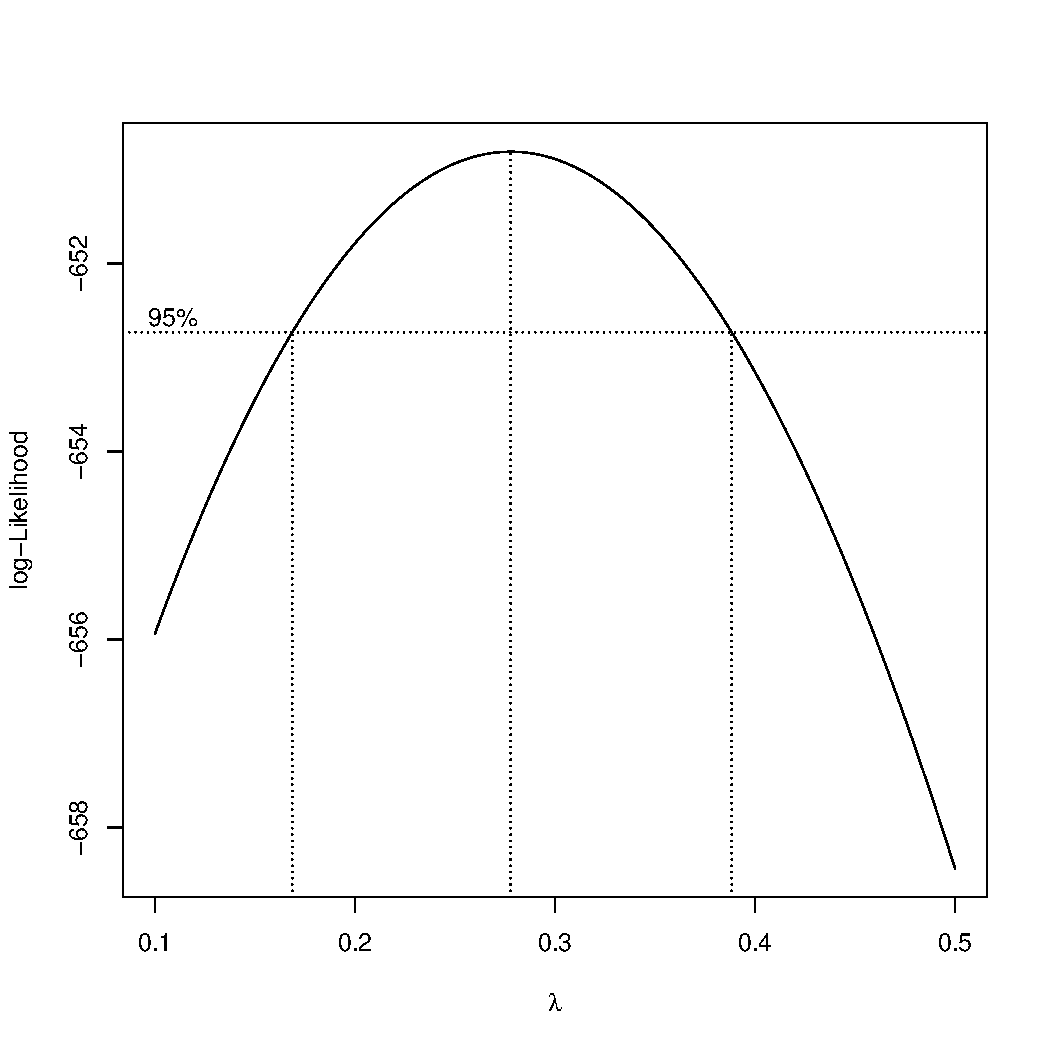
\includegraphics[width=10cm,height=10cm]{ozbxcx}
	\caption[ozone]{box cox potential for our response in ozone data}
	\label{ozonedata}
\end{figure}

the technical best transformation according to this graphic is 0.277778
\begin{verbatim}
	> temp = boxcox(ozMod, plotit=T, lambda=seq(0.10,0.5,by=0.1))
	> with(temp,x[which.max(y)])
	[1] 0.2777778
\end{verbatim}
However, for interperetability, I would pick .25
\item 9.5
We begin by looking at a boxcox transformation on the response. Doing so leads to the following graphic
\begin{figure}[H]
	\centering
	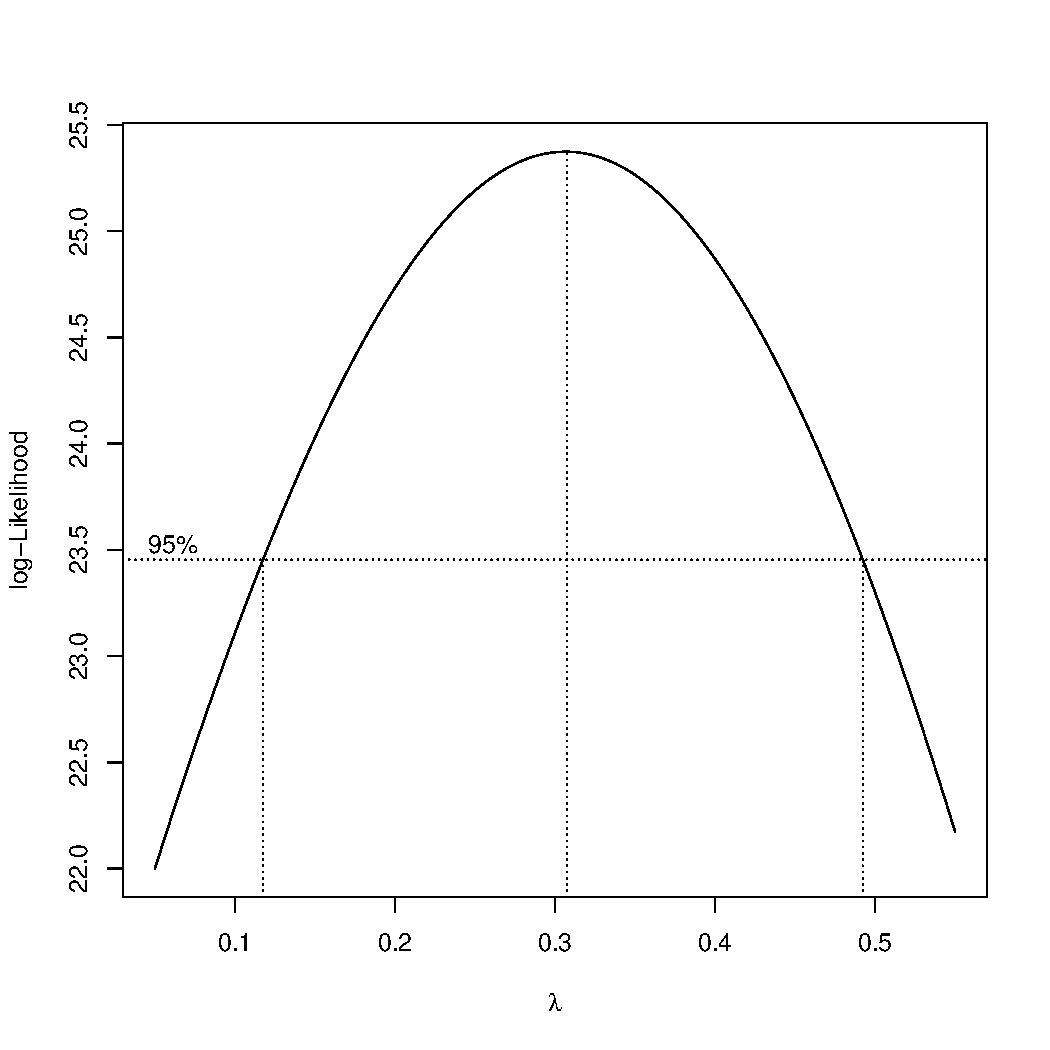
\includegraphics[width=10cm,height=10cm]{trbxcx}
	\caption[tree]{box cox potential for our response in tree data}
	\label{treedata}
\end{figure}
We see a value of about 1/3 seems appropriate. So we apply the transformation and get the following results
\begin{verbatim}
	> newTreemod = lm(((I(Volume^(1/3))-1)*3)~Girth+Height,treeData)
	> summary(treeModel)
	
	Call:
	lm(formula = Volume ~ Girth + Height, data = treeData)
	
	Residuals:
	Min      1Q  Median      3Q     Max 
	-6.4065 -2.6493 -0.2876  2.2003  8.4847 
	
	Coefficients:
	Estimate Std. Error t value Pr(>|t|)    
	(Intercept) -57.9877     8.6382  -6.713 2.75e-07 ***
	Girth         4.7082     0.2643  17.816  < 2e-16 ***
	Height        0.3393     0.1302   2.607   0.0145 *  
	---
	Signif. codes:  0 ‘***’ 0.001 ‘**’ 0.01 ‘*’ 0.05 ‘.’ 0.1 ‘ ’ 1
	
	Residual standard error: 3.882 on 28 degrees of freedom
	Multiple R-squared:  0.948,	Adjusted R-squared:  0.9442 
	F-statistic:   255 on 2 and 28 DF,  p-value: < 2.2e-16
	
	> summary(newTreemod)
	
	Call:
	lm(formula = ((I(Volume^(1/3)) - 1) * 3) ~ Girth + Height, data = treeData)
	
	Residuals:
	Min       1Q   Median       3Q      Max 
	-0.47881 -0.15060 -0.02048  0.20895  0.40194 
	
	Coefficients:
	Estimate Std. Error t value Pr(>|t|)    
	(Intercept) -3.256164   0.552944  -5.889 2.47e-06 ***
	Girth        0.454549   0.016916  26.871  < 2e-16 ***
	Height       0.043415   0.008331   5.211 1.56e-05 ***
	---
	Signif. codes:  0 ‘***’ 0.001 ‘**’ 0.01 ‘*’ 0.05 ‘.’ 0.1 ‘ ’ 1
	
	Residual standard error: 0.2485 on 28 degrees of freedom
	Multiple R-squared:  0.9777,	Adjusted R-squared:  0.9761 
	F-statistic: 612.5 on 2 and 28 DF,  p-value: < 2.2e-16
\end{verbatim}

Here we can see another slight improvement when making the box cox transformation.
\\
I examined if there were any non linear relationships between the predictors and the response, but there did not appear to be any so I stopped there.

\item  Finish R exercises 10.1, 10.4, 10.5, 10.6 of the textbook. Submit your
answers for {\color{red}ALL} questions. (For 10.1, use regsubsets() function in package "leaps" to do model selection based on Adjusted $R^2$ and Mallow's Cp; Use stepwise() function in package "Rcmdr" to do stepwise/forward/backward selection with  AIC and BIC.)
\item 10.1
\begin{enumerate}
	\item looking at our own backwards elimination, ill spare the details, but it comes down to a very simple model if we eliminate until nothing has over a 0.05 pvalue.
	\begin{verbatim}
		> sumary(pModel)
		Estimate Std. Error t value  Pr(>|t|)
		(Intercept) -0.268093   0.543500 -0.4933  0.622984
		lcavol       0.551638   0.074668  7.3879 6.304e-11
		lweight      0.508541   0.150170  3.3864  0.001039
		svi          0.666158   0.209777  3.1756  0.002029
		
		n = 97, p = 4, Residual SE = 0.71681, R-Squared = 0.63
	\end{verbatim}
	\item AIC
	\begin{figure}[H]
		\centering
		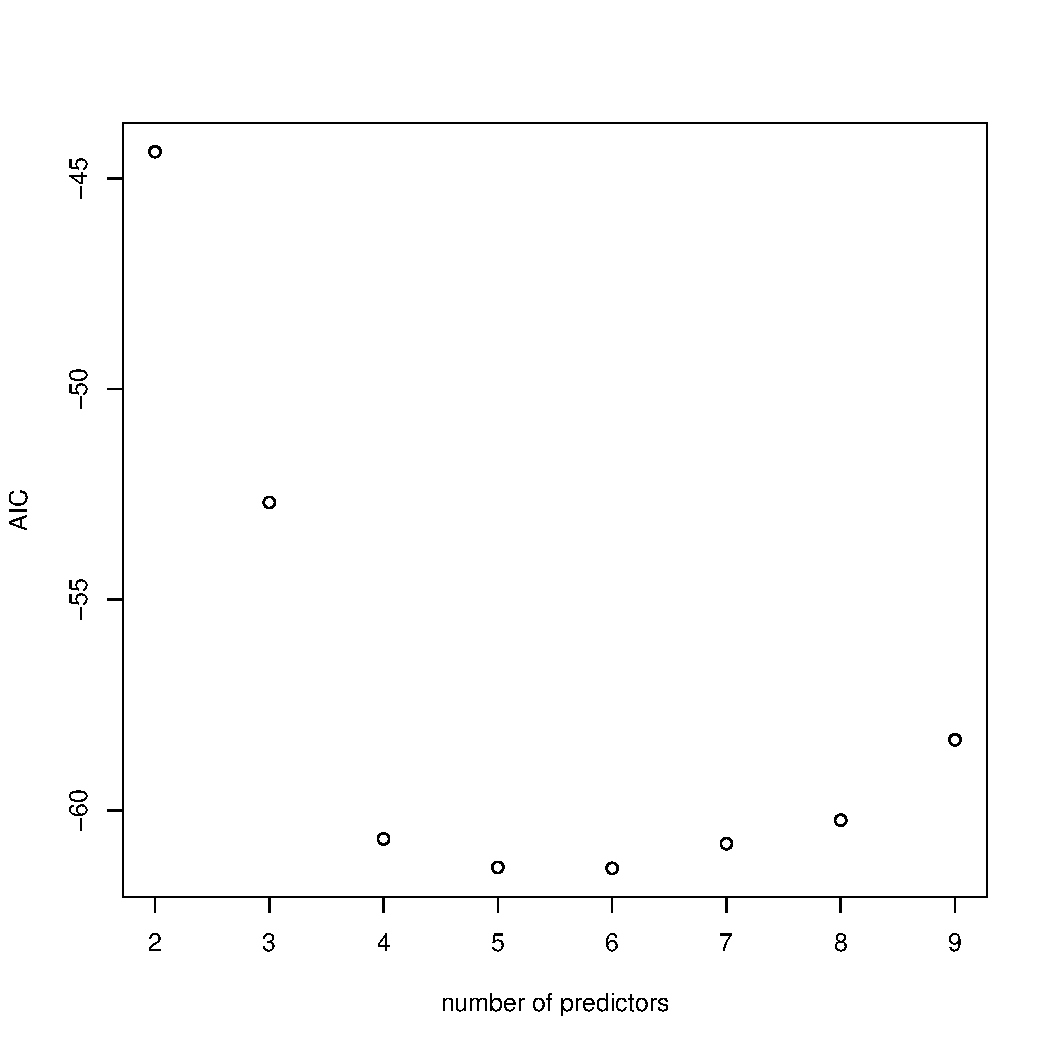
\includegraphics[width=10cm,height=10cm]{aicforprostate}
		\caption[paic]{graph of changing AIC scores as we add parameters}
		\label{aicp}
	\end{figure}
	looking at this, we can see our lowst AIC value occurs at about 5-6 predictors
	\item adjRsquared
	\begin{figure}[H]
		\centering
		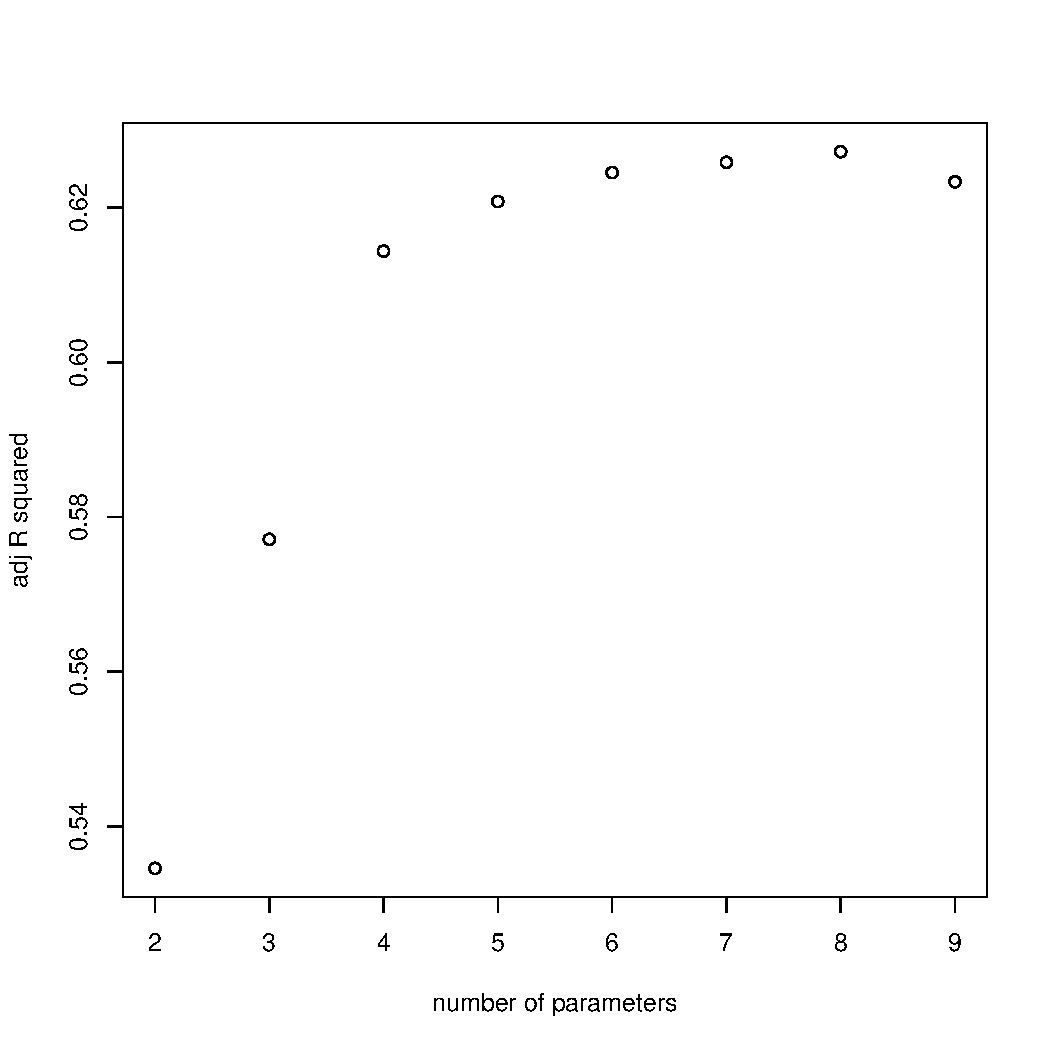
\includegraphics[width=10cm,height=10cm]{rsqrprostate}
		\caption[pr2]{graph of changing adjusted R squared scores as we add parameters}
		\label{adjr2}
	\end{figure}
	Unlike AIC, we are encouraged to take a slightly larger model at 8 parameters
	\item Cstats
	\begin{figure}[H]
		\centering
		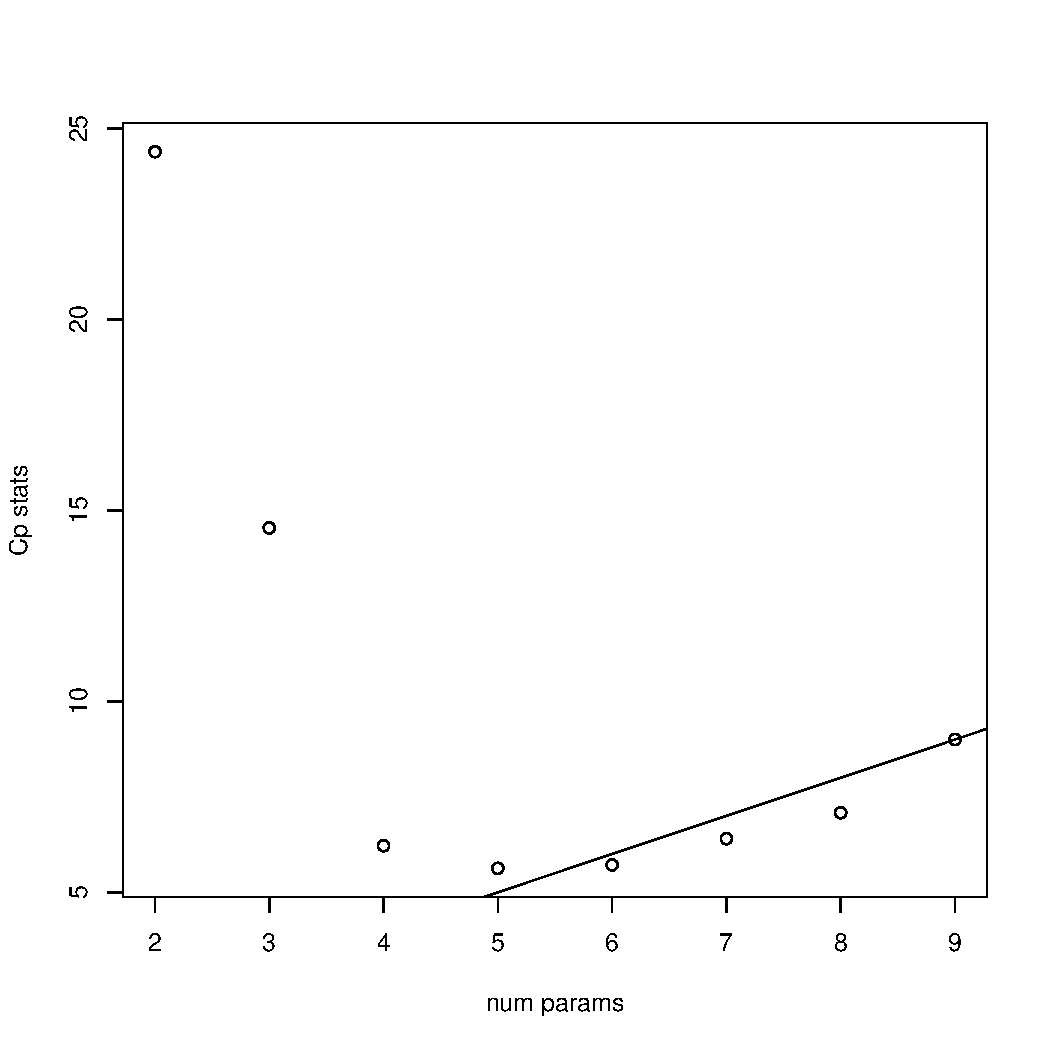
\includegraphics[width=10cm,height=10cm]{cstatprostate}
		\caption[pcstat]{c stat changes with increasing number of predictors}
		\label{cstat}
	\end{figure}
	This takes a bit more interpretation, but we are essentially choosing between 5 parameters and 9 parameters due to their closeness , but we may go with 5 predictors as it is a smaller model.
\end{enumerate}
	\item 10.4
	\begin{verbatim}
		 weirdTModel = lm(log(Volume)~I(Girth^2)+I(Height^2)+Height+Girth+Height*Girth,treeData)
		 > sumary(weirdTModel)
		 Estimate  Std. Error t value Pr(>|t|)
		 (Intercept)  -1.96602076  2.00669217 -0.9797 0.336605
		 I(Girth^2)   -0.00424100  0.00321830 -1.3178 0.199527
		 I(Height^2)  -0.00020220  0.00041859 -0.4831 0.633261
		 Height        0.04841962  0.05673214  0.8535 0.401498
		 Girth         0.28081258  0.07868562  3.5688 0.001485
		 Height:Girth -0.00019745  0.00180891 -0.1092 0.913950
		 
		 n = 31, p = 6, Residual SE = 0.08469, R-Squared = 0.98
	\end{verbatim}
	looking at these results, we can see there is a signifigant amount of repeated information, or at least, nothing is holding signifigance except for girth. I would say we cam simplify this by removing the higher order terms but keeping the interaction
	\begin{verbatim}
		> simplified= lm(log(Volume)~Height+Girth+Height*Girth,treeData)
		> sumary(simplified)
		Estimate  Std. Error t value  Pr(>|t|)
		(Intercept)  -2.14854241  0.74254835 -2.8935  0.007448
		Height        0.04530274  0.00965245  4.6934 6.943e-05
		Girth         0.33197647  0.05985482  5.5464 7.046e-06
		Height:Girth -0.00237961  0.00075942 -3.1335  0.004132
		
		n = 31, p = 4, Residual SE = 0.08438, R-Squared = 0.98
	\end{verbatim}
	We can see similar performance here, but now there is less complexity. There can be more exploration here but it will be refrained.
	\item 10.5
	\begin{verbatim}
		> sumary(smodel)
		Estimate Std. Error t value  Pr(>|t|)
		(Intercept) -39.91967   11.89600 -3.3557   0.00375
		Air.Flow      0.71564    0.13486  5.3066 5.799e-05
		Water.Temp    1.29529    0.36802  3.5196   0.00263
		Acid.Conc.   -0.15212    0.15629 -0.9733   0.34405
		
		n = 21, p = 4, Residual SE = 3.24336, R-Squared = 0.91
		> smodel2 = update(smodel,.~.-Acid.Conc.)
		> sumary(smodel2)
		Estimate Std. Error t value  Pr(>|t|)
		(Intercept) -50.35884    5.13833 -9.8006 1.216e-08
		Air.Flow      0.67115    0.12669  5.2976 4.898e-05
		Water.Temp    1.29535    0.36749  3.5249  0.002419
		
		n = 21, p = 3, Residual SE = 3.23862, R-Squared = 0.91
		> #point 21 is sorta suspect
		> pModelupd = lm(stack.loss~.,subset = temp < max(temp),sldata)
		> sumary(pModelupd)
		Estimate Std. Error t value  Pr(>|t|)
		(Intercept) -43.70403    9.49157 -4.6045  0.000293
		Air.Flow      0.88911    0.11885  7.4811 1.309e-06
		Water.Temp    0.81662    0.32503  2.5124  0.023088
		Acid.Conc.   -0.10714    0.12454 -0.8603  0.402338
		
		n = 20, p = 4, Residual SE = 2.56920, R-Squared = 0.95
		> smodelupd2 = update(pModelupd,.~.-Acid.Conc.)
		> sumary(smodelupd2)
		Estimate Std. Error  t value  Pr(>|t|)
		(Intercept) -51.07598    4.05024 -12.6106 4.692e-10
		Air.Flow      0.86300    0.11403   7.5684 7.701e-07
		Water.Temp    0.80326    0.32217   2.4933   0.02326
		
		n = 20, p = 3, Residual SE = 2.54949, R-Squared = 0.95
	\end{verbatim}
	The analysis for outliers and influential points was removed. Essentially, looking at leverages, cooks distance, and studentized residuals. Data point 21 stood out. It was subsequently removed and we see a signifigant improvement in out R squared, but each the variable selection process remains the same and Acid.Conc. is removed as it is not needed in either model with or without the outlier.
	\item 10.6
	\begin{verbatim}
		> spModel = lm(hipcenter~.,spData)
		> sumary(spModel)
		Estimate Std. Error t value Pr(>|t|)
		(Intercept) 436.432128 166.571619  2.6201  0.01384
		Age           0.775716   0.570329  1.3601  0.18427
		Weight        0.026313   0.330970  0.0795  0.93718
		HtShoes      -2.692408   9.753035 -0.2761  0.78446
		Ht            0.601345  10.129874  0.0594  0.95307
		Seated        0.533752   3.761894  0.1419  0.88815
		Arm          -1.328069   3.900197 -0.3405  0.73592
		Thigh        -1.143119   2.660024 -0.4297  0.67056
		Leg          -6.439046   4.713860 -1.3660  0.18245
		
		n = 38, p = 9, Residual SE = 37.72029, R-Squared = 0.69
	\end{verbatim}
	a) it appears that initially, the leg has a decent amount of explaining power despite the many other predictors present. This is not statistically signifigant at the 0.05 level, but we can generally say that as we increase the length of our legs, the hip center is shifted negatively assuming all other variables remain constant.
	\\
	b)
	\begin{verbatim}
		> means
		[1]  35.26316 155.63158 171.38947 169.08421  88.95263  32.21579  38.65526  36.26316
		> predict(spModel,new=data.frame(Age=means[1],Weight=means[2],
		HtShoes=means[3],Ht=means[4],Seated=means[5],Arm=means[6],
		Thigh=means[7],Leg=means[8]),interval="prediction")
		fit     lwr       upr
		1 -164.8849 -243.04 -86.72972
	\end{verbatim}
	means were computed manually via a for loop visible in the R code.
	\\
	c)
	\begin{verbatim}
		> holdon$anova
		Stepwise Model Path 
		Analysis of Deviance Table
		
		Initial Model:
		hipcenter ~ Age + Weight + HtShoes + Ht + Seated + Arm + Thigh + 
		Leg
		
		Final Model:
		hipcenter ~ Age + HtShoes + Leg
		
		
		Step Df   Deviance Resid. Df Resid. Dev      AIC
		1                               29   41261.78 283.6240
		2     - Ht  1   5.014051        30   41266.80 281.6286
		3 - Weight  1  11.103872        31   41277.90 279.6389
		4 - Seated  1  35.096713        32   41313.00 277.6712
		5    - Arm  1 172.016420        33   41485.01 275.8291
		6  - Thigh  1 472.777374        34   41957.79 274.2597
	\end{verbatim}
	fitting a final model to this we get 
	\begin{verbatim}
		> finalModel = lm(hipcenter~Age+HtShoes+Leg,spData)
		> sumary(finalModel)
		Estimate Std. Error t value  Pr(>|t|)
		(Intercept) 456.21365  102.80779  4.4375 9.092e-05
		Age           0.59983    0.37792  1.5872   0.12173
		HtShoes      -2.30226    1.24520 -1.8489   0.07318
		Leg          -6.82975    4.06926 -1.6784   0.10244
		
		n = 38, p = 4, Residual SE = 35.12909, R-Squared = 0.68
	\end{verbatim}
	This time, we are still not confident in our answer, but we are more confident now. It is still negative a will shift the hip center negatively given a positive change in leg values while all else is held constant. We get the following prediction interval
	\begin{verbatim}
		> predict(finalModel,new=data.frame(Age=means[1],HtShoes=means[3],
		Leg=means[8]),interval="prediction")
		fit      lwr       upr
		1 -164.8849 -237.209 -92.56072
	\end{verbatim}
	As we can see, there is a similar fit between the two models, however, our confidence interval is actually narrower than our prior estimate.
\end{enumerate}

\end{document}
